% Q19：对角线依次落在 x 轴并首尾相接的正方形；非比例示意。
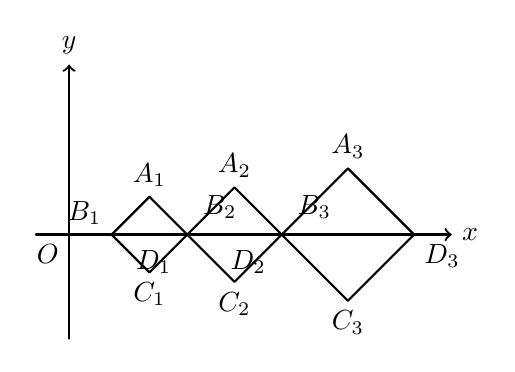
\begin{tikzpicture}[line cap=round,line join=round,thick,scale=1.2]
  \coordinate (Bone) at (0.45,0);
  \coordinate (Done) at (1.25,0);
  \coordinate (Aone) at (0.85,0.4);
  \coordinate (Cone) at (0.85,-0.4);
  \coordinate (Btwo) at (1.25,0);
  \coordinate (Dtwo) at (2.25,0);
  \coordinate (Atwo) at (1.75,0.5);
  \coordinate (Ctwo) at (1.75,-0.5);
  \coordinate (Bthree) at (2.25,0);
  \coordinate (Dthree) at (3.65,0);
  \coordinate (Athree) at (2.95,0.7);
  \coordinate (Cthree) at (2.95,-0.7);

  \draw[->] (-0.35,0)--(4.05,0) node[right] {$x$};
  \draw[->] (0,-1.1)--(0,1.8) node[above] {$y$};
  \draw (Bone)--(Aone)--(Done)--(Cone)--cycle;
  \draw (Btwo)--(Atwo)--(Dtwo)--(Ctwo)--cycle;
  \draw (Bthree)--(Athree)--(Dthree)--(Cthree)--cycle;

  \node[below left] at (0,0) {$O$};
  \node[above left] at (Bone) {$B_1$};
  \node[above] at (Aone) {$A_1$};
  \node[below] at (Cone) {$C_1$};
  \node[below left,xshift=-2pt,yshift=-2pt] at (Done) {$D_1$};
  \node[above right,xshift=2pt,yshift=2pt] at (Btwo) {$B_2$};
  \node[above] at (Atwo) {$A_2$};
  \node[below] at (Ctwo) {$C_2$};
  \node[below left,xshift=-2pt,yshift=-2pt] at (Dtwo) {$D_2$};
  \node[above right,xshift=2pt,yshift=2pt] at (Bthree) {$B_3$};
  \node[above] at (Athree) {$A_3$};
  \node[below] at (Cthree) {$C_3$};
  \node[below right] at (Dthree) {$D_3$};
\end{tikzpicture}
